%----------------------------------------------------------
\def\notedate{2023.05.04}
\def\currentauthor{Василян А.Р. (РК6-83Б)}
%----------------------------------------------------------
\notestatement{rndhpcgui}{Генерация страницы на основе данных в формате aINI.}

%---------------------------------------------------------


Была разработана программа для преобразования данных формата \textsf{aINI} в \textsf{HTML}-код. Во время разработки программы преобразования данных из \textsf{aINI} в \textsf{HTML} использовался модуль синтаксического анализа для языка \textsf{Python} - \textsf{Pyparsing}. 

После запуска программа в функции \textsf{main} (листинг~\ref{rndhpcgui.2023.05.04.main}) считывает построчно данные из файла \textsf{config} (пример содержимого файла \textsf{config} на листинге ~\ref{rndhpcgui.2023.05.04.config}). В данном файле представленые в квадратных скобках названия искомых файлов, на основе которых будут генерироваться \textsf{HTML}-страницы (содержимое такого файла представлено на листинге ~\ref{rndhpcgui.2023.05.04.input1}), до знака "=" - \textsf{URL} для соответсвующей страницы, а после "//" наименование страницы. На основе файла \textsf{config} также будет создана страница menu, из которой можно будет перейти на все страницы, перечисленные в \textsf{config}. В функции \textsf{main} создаются ещё два текстовых файла: \textsf{txt_for_urls}, \textsf{txt_for_views}. В этих файлах будет записан дополнительный код, который пользователю необходимо будет вставить в соответствующие файлы в \textsf{web}-приложения для корректного взаимодействия приложения с \textsf{HTML}-файлами (в комментариях в файлах присутствует информация о том, куда должен быть скопирован код). Пример файлов \textsf{txt_for_urls} и \textsf{txt_for_views} представлен на рис.~\ref{rndhpcgui.2023.05.04.picture1}. Наименование страницы и название файла с данными формата \textsf{aINI} считанные из \textsf{config} передаются функции \textsf{aini_to_html}(листинг~\ref{rndhpcgui.2023.02.28.aini_to_html}).


\begin{lstlisting}[frame=single, label={rndhpcgui.2023.05.04.main}, caption={Функция main}, language={Python}] 
    def main():
    input_f = open('input/config', encoding='utf-8')
    f_menu = open(r'output\menu.html', 'w', encoding='utf-8')
    f_urls = open(r'output\txt_for_urls.txt', 'w', encoding='utf-8')
    f_views = open(r'output\txt_for_views.txt', 'w', encoding='utf-8')
    list_of_functions = 'from upload.views import menu'

    f_urls.write('//Ниже представлен код, который должен быть вставлен в файл urls.py в список urlpatterns\n\n\tpath('
                 '"", menu, name="menu"),\n')
    f_views.write(
        '//Ниже представлен код, который должен быть вставлен в файл views.py\n\ndef menu(request):\n\treturn render('
        'request, "menu.html")\n\n')
    f_menu.write(
        '<!DOCTYPE html>\n<html lang="en">\n<head>\n<meta charset="UTF-8">\n<style>\nbody {font-family: '
        'Arial;}\n\n.tab {\n\toverflow: hidden;\n\tborder: 1px solid #ccc;\n\tbackground-color: #f1f1f1;\n}\n\n.tab '
        'button {\n\toverflow: hidden;\n\tborder: 1px solid #ccc;\n\tbackground-color: #ddd;\n\tfloat: left;\n\tborder: '
        'none;\n\toutline: none;\n\tcursor: pointer;\n\tpadding: 14px 16px;\n\ttransition: 0.3s;\n\tfont-size: '
        '17px;\n\tdisplay: block;\n\twidth: 100%;\n}\n\n.tab button:hover {\n\tbackground-color: '
        '#808080;\n}\n\n</style>\n<title>menu</title>\n</head>\n<body>\n<h1>Здравствуйте! Выберите один из '
        'предложенных вариантов.</h1>\n<div class="tab">\n')

    for line in input_f:
        global num_of_section
        num_of_section = -1

        try:
            config = aini_file_name.parseString(line).asList()
        except ParseException:
            print('The string is not parsed: ')
            print(line)
            quit()

        f_menu.write('\t<button onclick="document.location=\'/' + config[0] + '/\'">' + config[6] + '</button>\n')
        f_urls.write('\tpath("' + config[0] + '/", ' + config[3] + ', name="' + config[3] + '"),\n')
        list_of_functions = list_of_functions + ', ' + config[3]
        list_of_variables = aini_to_html(config[3], config[6])
        f_views.write('def ' + config[3] + '(request):\n\tif request.method == "POST":\n')

        for variable in list_of_variables:
            f_views.write(variable)

        f_views.write('\t\treturn render(request, "' + config[3] + '.html")\n\treturn render(request, "' + config[
            3] + '.html")\n\n')

    f_menu.write('</div>\n</body>\n</html>\n')
    f_urls.write('\n//Также вставьте следующую строку в файл urls.py до списка urlpatterns\n' + list_of_functions)
\end{lstlisting}

\begin{figure}[!ht]
    \centering
    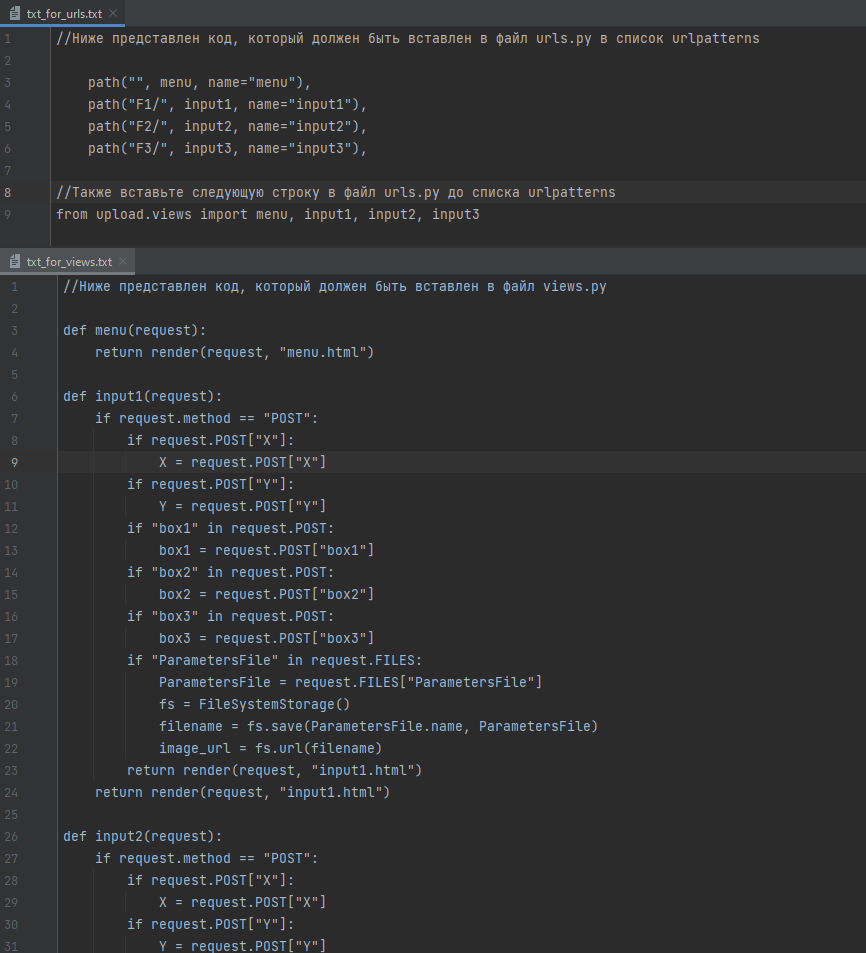
\includegraphics[scale=0.7]{ResearchNotes/rndhpc_dev_gui_2023_05_04/rndhpcgui.2023.05.04.picture1.png}
    \caption{Пример файлов txt_for_urls, txt_for_views}
    \label{rndhpcgui.2023.05.04.picture1}
\end{figure}


В функции \textsf{aini_to_html}(листинг~\ref{rndhpcgui.2023.02.28.aini_to_html}) построчно считываются данные из \textsf{aINI} файла и распознает строку в соответствии с шаблонами в парсере (листинг~\ref{rndhpcgui.2023.05.04.parser}). При использовании pyparsing, парсер вначале был написан для отдельных ключевых элементов (например ссылка, текст из английских и русских букв и тп.), а потом из отдельных частей получается парсер для всей строки \textsf{aINI}-кода. Расспознавание строк происходит в функции parsing (листинг~\ref{rndhpcgui.2023.05.04.parsing}), которая возвращает список из распознанных частей строки и номер распознанного элемента интерфейса для дальнещей генерации.


На основе списка и номера элемента интерфейса создается \textsf{HTML}-код с помощью вызова соответствующей функции для каждого из предусмотренных элементов интерфейса (листинг~\ref{rndhpcgui.2023.05.04.generation}). Для некоторых элементов интерфейса (окно для ввода текста, флажок, выбор файла и тп.) функция создания \textsf{HTML}-кода возвращает код для функции представленния, который далее будет выведен в ранее упомянутый файл \textsf{txt_for_views}.

\begin{lstlisting}[frame=single, label={rndhpcgui.2023.05.04.parser}, caption={Парсер}, language={Python}] 
    rus_alphas = 'ёйцукенгшщзхъфывапролджэячсмитьбюЁЙЦУКЕНГШЩЗХЪФЫВАПРОЛДЖЭЯЧСМИТЬБЮ'

    bool_var = Word('0' + '1')
    word_num = Word(nums + alphas)
    variable = Word(nums + alphas + '_')
    rus_eng_word_num = Word(alphas + rus_alphas + ' ' + nums)
    link = Word(alphanums + '-' + '+' + '=' + '/' + '.' + '_' + '#' + ':' + '&' + '?' + '%')
    text = Word(printables + rus_alphas + ' ')
    menu_link = Word(alphanums + '-' + '+' + '=' + '.' + '_' + '#' + ':' + '&' + '?' + '%')
    
    parse_section = '[' + variable + ']' + '//' + rus_eng_word_num
    parse_text_box = variable + '=' + word_num + '//' + rus_eng_word_num
    parse_box = variable + '=' + '[' + bool_var + ']' + '{0|1}' + '//' + rus_eng_word_num
    parse_file_selection = variable + '=' + '[file]' + '//' + rus_eng_word_num
    parse_link = '[' + link + ']' + '//' + rus_eng_word_num
    parse_text = '//' + OneOrMore(text)
    aini_file_name = menu_link + '=' + '[' + variable + ']' + '//' + rus_eng_word_num
\end{lstlisting}

\begin{lstlisting}[frame=single, label={rndhpcgui.2023.05.04.parsing}, caption={Функция parsing}, language={Python}] 
    def parsing(s):
    try:
        test = parse_section.parseString(s).asList()
        patern_id = 1
    except ParseException:
        try:
            test = parse_text_box.parseString(s).asList()
            patern_id = 2
        except ParseException:
            try:
                test = parse_box.parseString(s).asList()
                patern_id = 3
            except ParseException:
                try:
                    test = parse_file_selection.parseString(s).asList()
                    patern_id = 4
                except ParseException:
                    try:
                        test = parse_link.parseString(s).asList()
                        patern_id = 5
                    except ParseException:
                        try:
                            test = parse_text.parseString(s).asList()
                            patern_id = 6
                        except ParseException:
                            print('The string is not parsed:' + s + '')
                            quit()
    return [patern_id, test]
\end{lstlisting}

\begin{lstlisting}[frame=single, label={rndhpcgui.2023.05.04.aini_to_html}, caption={Функция aini_to_html}, language={Python}] 
    def aini_to_html(file_name, title):
    sections_list = []
    elements_list = []
    list_of_variables = []

    input_f = open('input/' + file_name, encoding='utf-8')
    f = html_start(title, file_name)

    for line in input_f:
        id_and_line = parsing(line)
        patern_id = id_and_line[0]
        parsed_line = id_and_line[1]
        if patern_id <= 3:
            match patern_id:
                case 1:
                    html_code = section_to_html(parsed_line)
                    sections_list.append(html_code)
                case 2:
                    html_code = textbox_to_html(parsed_line)
                    if len(elements_list) == num_of_section + 1:
                        elements_list[num_of_section] += html_code[1]
                    else:
                        elements_list.append(html_code[1])
                    list_of_variables.append(html_code[0])
                case 3:
                    html_code = box_to_html(parsed_line)
                    if len(elements_list) == num_of_section + 1:
                        elements_list[num_of_section] += html_code[1]
                    else:
                        elements_list.append(html_code[1])
                    list_of_variables.append(html_code[0])
        else:
            match patern_id:
                case 4:
                    html_code = file_selection_to_html(parsed_line)
                    if len(elements_list) == num_of_section + 1:
                        elements_list[num_of_section] += html_code[1]
                    else:
                        elements_list.append(html_code[1])
                    list_of_variables.append(html_code[0])
                case 5:
                    html_code = link_to_html(parsed_line)
                    if len(elements_list) == num_of_section + 1:
                        elements_list[num_of_section] += html_code
                    else:
                        elements_list.append(html_code)
                case 6:
                    html_code = text_to_html(parsed_line)
                    if len(elements_list) == num_of_section + 1:
                        elements_list[num_of_section] += html_code
                    else:
                        elements_list.append(html_code)

    for section in sections_list:
        f.write(section)
    f.write('</div>\n\n')

    i = 0
    f.write('<form method="post" enctype="multipart/form-data">\n\n\n')
    for element in elements_list:
        id = 'section_' + str(i)
        f.write('<div id="' + id + '" class="tabcontent">\n' + element + '</div>\n\n')
        i += 1
    html_finish(f)
    return list_of_variables
\end{lstlisting}

\begin{lstlisting}[frame=single, label={rndhpcgui.2023.05.04.generation}, caption={Функции создания HTML-кода}, language={Python}] 
    def section_to_html(parsed_line):
    if len(parsed_line) != 5:
        section = parsed_line[1]
    else:
        section = parsed_line[4]
    global num_of_section
    num_of_section += 1
    id = "'section_" + str(num_of_section) + "'"
    if num_of_section == 0:
        return '\t<button class="tablinks" onclick="tabs(event,' + id + ')" id="defaultOpen">' + section + '</button>\n'
    else:
        return '\t<button class="tablinks" onclick="tabs(event,' + id + ')">' + section + '</button>\n'


def textbox_to_html(parsed_line):
    html_code = []
    if len(parsed_line) != 5:
        textbox = parsed_line[0]
    else:
        textbox = parsed_line[4]
    html_code.append('\t\tif request.POST["' + parsed_line[0] + '"]:\n\t\t\t' + parsed_line[0] + ' = request.POST["' + parsed_line[0] + '"]\n')
    html_code.append('\t<p><b>' + textbox + '</b><br>\n\t<input type="text" name="' + parsed_line[0] + '" value="' + parsed_line[2] + '"></p>\n')
    return html_code


def box_to_html(parsed_line):
    html_code = []
    if len(parsed_line) != 8:
        box = parsed_line[0]
    else:
        box = parsed_line[7]
    html_code.append('\t\tif "' + parsed_line[0] + '" in request.POST:\n\t\t\t' + parsed_line[0] + ' = request.POST["' + parsed_line[0] + '"]\n')
    if parsed_line[3] == '1':
        html_code.append('\t<p><<input type="checkbox" name="' + parsed_line[0] + '" value="' + parsed_line[0] + '" checked>' + box + '</p>\n')
    else:
        html_code.append('\t<p><<input type="checkbox" name="' + parsed_line[0] + '" value="' + parsed_line[0] + '">' + box + '</p>\n')
    return html_code


def file_selection_to_html(parsed_line):
    html_code = []
    if len(parsed_line) != 5:
        file_selection = parsed_line[0]
    else:
        file_selection = parsed_line[4]
    html_code.append('\t\tif "' + parsed_line[0] + '" in request.FILES:\n\t\t\t' + parsed_line[0] + ' = request.FILES["' + parsed_line[0] + '"]\n\t\t\tfs = FileSystemStorage()\n\t\t\tfilename = fs.save(' + parsed_line[0] + '.name, ' + parsed_line[0] + ')\n\t\t\tfile_url = fs.url(filename)\n')
    html_code.append('\t<p><b>' + file_selection + '</b><br>\n\t<input type="file" name="' + parsed_line[0] + '"></p>\n')
    return html_code


def link_to_html(parsed_line):
    if len(parsed_line) != 5:
        link_title = parsed_line[1]
    else:
        link_title = parsed_line[4]
    return '\t<p><a href="' + parsed_line[1] + '">' + link_title + '</a></p>\n'


def text_to_html(parsed_line):
    return '\t<p>' + parsed_line[1] + '</p>\n'

\end{lstlisting}


Пример входных данных программы представлены на листингах~\ref{rndhpcgui.2023.05.04.config} (файл \textsf{config}),~\ref{rndhpcgui.2023.05.04.input1}(один из трёх файлов, на которых указывает \textsf{config}). 

\begin{lstlisting}[frame=single, label={rndhpcgui.2023.05.04.config}, caption={config}, language={aINIExample}] 
    F1 = [input1]//Test1
    F2 = [input2]//Test2
    F3 = [input3]//Test3
\end{lstlisting}

\begin{lstlisting}[frame=single, label={rndhpcgui.2023.05.04.input1}, caption={input1}, language={aINIExample}] 
    [sec1]//Пункт 1
    X=VX//Параметр X
    Y=25//Параметр Y
    box1=[1] {0|1}//Флажок 1
    box2=[1] {0|1}//Флажок 2
    [sec2]//Пункт 2
    box3=[0] {0|1}//Флажок 3
    ParametersFile=[file]//Выберите имя файла
    [https://www.google.ru]//Ссылка на Google
    //Московский государственный технический университет им. Н. Э. Баумана - российский национальный исследовательский университет, научный центр, особо ценный объект культурного наследия народов России.
\end{lstlisting}


Пример выходных данных программы представлены на листингах~\ref{rndhpcgui.2023.05.04.menu} (главное меню, созданное на основе \textsf{config}), ~\ref{rndhpcgui.2023.05.04.input1_html}({HTML}-код первой из трёх страниц), рис.~\ref{rndhpcgui.2023.05.04.picture1} (файлы с дополнительным необходимым кодом txt_for_urls, txt_for_views).
\begin{lstlisting}[frame=single, label={rndhpcgui.2023.05.04.menu}, caption={Главное меню}, language={HTML}] 
    <!DOCTYPE html>
    <html lang="en">
    <head>
    <meta charset="UTF-8">
    <style>
    body {font-family: Arial;}
    
    .tab {
        overflow: hidden;
        border: 1px solid #ccc;
        background-color: #f1f1f1;
    }
    
    .tab button {
        overflow: hidden;
        border: 1px solid #ccc;
        background-color: #ddd;
        float: left;
        border: none;
        outline: none;
        cursor: pointer;
        padding: 14px 16px;
        transition: 0.3s;
        font-size: 17px;
        display: block;
        width: 100%;
    }
    
    .tab button:hover {
        background-color: #808080;
    }
    
    </style>
    <title>menu</title>
    </head>
    <body>
    <h1>Здравствуйте! Выберите один из предложенных вариантов.</h1>
    <div class="tab">
        <button onclick="document.location='/F1/'">Test1</button>
        <button onclick="document.location='/F2/'">Test2</button>
        <button onclick="document.location='/F3/'">Test3</button>
    </div>
    </body>
    </html>
    
\end{lstlisting}

\begin{lstlisting}[frame=single, label={rndhpcgui.2023.05.04.input1_html}, caption={Главное меню}, language={HTML}] 
    <!DOCTYPE html>
    <html>
    <head>
    <meta name="viewport" content="width=device-width, initial-scale=1">
    <style>
    body {font-family: Arial;}
    
    .tab {
        overflow: hidden;
        border: 1px solid #ccc;
        background-color: #f1f1f1;
    }
    
    .tab button, .clickable {
        float: left;
    border: none;
        outline: none;
        cursor: pointer;
        padding: 14px 16px;
        transition: 0.3s;
        font-size: 17px;
    }
    
    .tab button:hover, .clickable:hover {
        background-color: #ddd;
    }
    
    .tab button.active {
        background-color: #ccc;
    }
    
    .tabcontent {
        display: none;
        padding: 6px 12px;
        border: 1px solid #ccc;
        border-top: none;
    }
    </style>
    <title>Test1</title>
    </head>
    <body>
     
    <div class="tab">
        <button class="tablinks" onclick="tabs(event,'section_0')" id="defaultOpen">Пункт 1</button>
        <button class="tablinks" onclick="tabs(event,'section_1')">Пункт 2</button>
    </div>
    
    <form method="post" enctype="multipart/form-data">
    
    
    <div id="section_0" class="tabcontent">
        <p><b>Параметр X</b><br>
        <input type="text" name="X" value="VX"></p>
        <p><b>Параметр Y</b><br>
        <input type="text" name="Y" value="25"></p>
        <p><<input type="checkbox" name="box1" value="box1" checked>Флажок 1</p>
        <p><<input type="checkbox" name="box2" value="box2" checked>Флажок 2</p>
    </div>
    
    <div id="section_1" class="tabcontent">
        <p><<input type="checkbox" name="box3" value="box3">Флажок 3</p>
        <p><b>Выберите имя файла</b><br>
        <input type="file" name="ParametersFile"></p>
        <p><a href="https://www.google.ru">Ссылка на Google</a></p>
        <p>Московский государственный технический университет им. Н. Э. Баумана - российский национальный исследовательский университет, научный центр, особо ценный объект культурного наследия народов России.</p>
    </div>
    
    <p><input class="clickable" type="submit"></p>
    </form>
    <br>
    <br>
    <br>
    <button class="clickable" onclick="document.location='/'">Назад</button>
    
    <script>
    function tabs(evt, tab_id) {
        var i, tabcontent, tablinks;
        tabcontent = document.getElementsByClassName("tabcontent");
        for (i = 0; i < tabcontent.length; i++) {
            tabcontent[i].style.display = "none";
        }
        tablinks = document.getElementsByClassName("tablinks");
        for (i = 0; i < tablinks.length; i++) {
            tablinks[i].className = tablinks[i].className.replace(" active", "");
        }
        document.getElementById(tab_id).style.display = "block";
        evt.currentTarget.className += " active";
    }
    
    document.getElementById("defaultOpen").click();
    </script>
    
    </body>
    </html>
\end{lstlisting}

Полученные файлы и код были добавленны в ранее реализованное \textsf{web}-приложение. Демонстрация работы \textsf{web}-приложения с новым интерфейсом представлена на рис.~\ref{rndhpcgui.2023.05.04.picture2} и рис.~\ref{rndhpcgui.2023.05.04.picture3}

\begin{figure}[!ht]
    \centering
    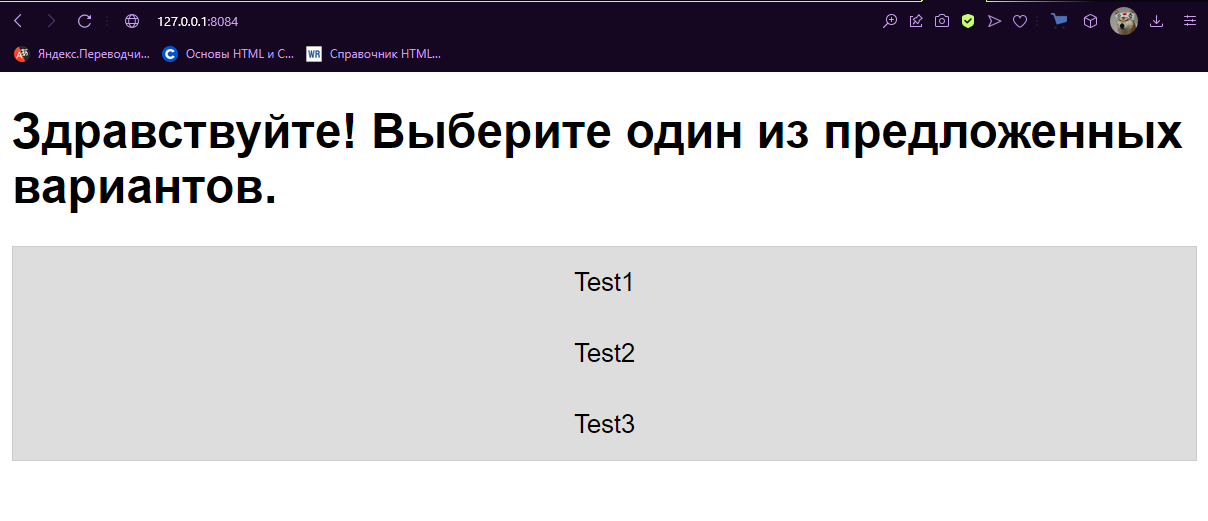
\includegraphics[scale=0.5]{ResearchNotes/rndhpc_dev_gui_2023_05_04/rndhpcgui.2023.05.04.picture2.png}
    \caption{Главное меню в web-приложении}
    \label{rndhpcgui.2023.05.04.picture2}
\end{figure}

\begin{figure}[!ht]
    \centering
    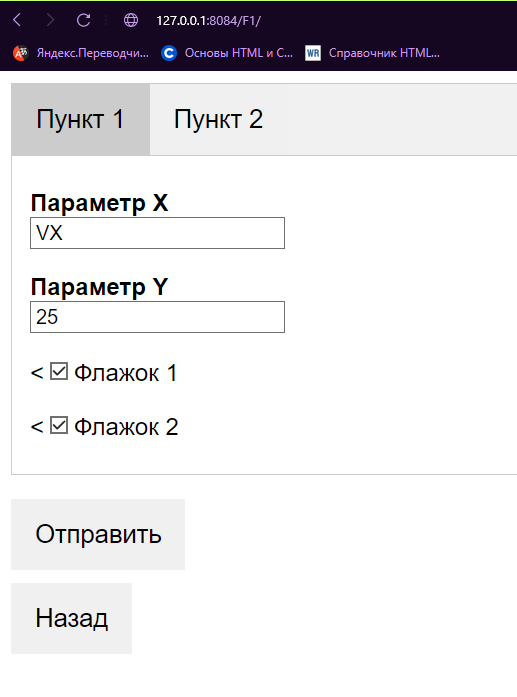
\includegraphics[scale=0.6]{ResearchNotes/rndhpc_dev_gui_2023_05_04/rndhpcgui.2023.05.04.picture3.png}
    \caption{Одна из страниц web-приложения}
    \label{rndhpcgui.2023.05.04.picture3}
\end{figure}

Для демонстрации того, что введённые данные сохранаются, код страницы был изменён, чтобы вывести введённые данные после отправки. Результат представлен на рис.~\ref{rndhpcgui.2023.05.04.picture4}

\begin{figure}[!ht]
    \centering
    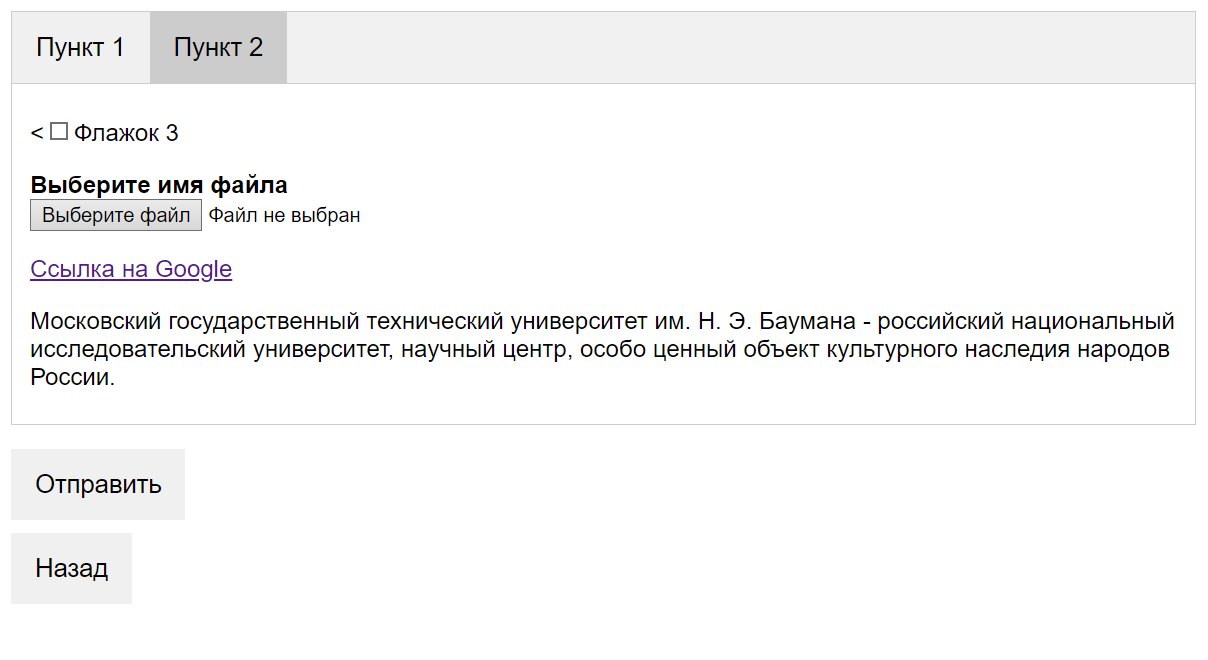
\includegraphics[scale=0.5]{ResearchNotes/rndhpc_dev_gui_2023_05_04/rndhpcgui.2023.05.04.picture4.png}
    \caption{Вывод введённых данных}
    \label{rndhpcgui.2023.05.04.picture4}
\end{figure}
%----------------------------------------------------------
% Атрибуты задачи
\noteattributes{}
%----------------------------------------------------------
